\chapter{Diseño experimental}
\label{chap:metodologia_experimental}

%% como se mide y bajo que entorno

%% bencharmk cec2017
%% dimension, presupeusto, semillas, rango
%% mirar tfgs previos 
%% métricas
%% detalles de implemetacion experimental
%% protocolo de ajuste fino, 

%% configuracion para las estrategias offline con los porcentajes tenidos en cuenta

%% configuraciones evaluadas para el criterio de reinicio: sin reinico y ventanas candidatas.

%% hay que adaptarlo cuando vayamos incrementando el contenido experimental: ahora mismo solo referencia a las dos estrategias offline que vamos a evaluar.

En este capítulo se recoge el protocolo experimental seguido para evaluar las técnicas subrogadas consideradas en este trabajo y su integración en el bucle de optimización.

Para ello, se presenta en primer lugar el benchmark utilizado y se detallan las condiciones bajo las que se ejecutan las metaheurísticas. A continuación, se describen las técnicas subrogadas consideradas y las transformaciones aplicadas a los datos antes de su entrenamiento.
Posteriormente, se definen las estrategias de evaluación, las métricas empleadas y el criterio seguido para comparar los modelos. Finalmente, se documentan de forma separada los detalles de implementación y el entorno necesario para reproducir las ejecuciones.

%%%%%%%%%%%%%%%%%%%%%%
\section{Benchmark utilizado}
\label{sec:benchmark}

La evaluación experimental de una metaheurística requiere disponer de un
conjunto de problemas que permita comparar su comportamiento bajo condiciones
homogéneas. En este trabajo se utiliza la suite \textbf{CEC2017}, propuesta para la
\textit{Special Session and Competition on Single Objective Bound Constrained
    Real-Parameter Numerical Optimization} del IEEE Congress on Evolutionary
Computation de 2017~\cite{awad2017cec2017}.

\subsection{Suite CEC2017}
\label{subsec:suite_cec2017}

% Describe brevemente las familias de funciones, el dominio de búsqueda y el carácter continuo y monoobjetivo del benchmark.


%% se pueden mostrar dos imágenes que representen el paisaje de dos funciones muy distintas en CEC para decir algo como: se puede ver que muestran un paisaje muy distinto y que cada problema de optimizacion es distinto

%% pero no vamos a utilizar una tabla que muestre TODAS las funciones (30 funcinoes) que componen a cec2017.

\textbf{CEC2017} está formada por problemas de optimización continua,
monoobjetivo y con variables acotadas. Cada solución candidata se representa
mediante un vector \(\mathbf{x} \in [-100,100]^D\), donde \(D\) indica la
dimensión del problema.

Las funciones que la componen plantean escenarios de optimización con distintos niveles de dificultad y se agrupan en cuatro familias según las características de su paisaje de búsqueda:

\begin{itemize}
    \item \textbf{Funciones unimodales}: permiten analizar la capacidad de
          convergencia de los algoritmos en problemas con una única región óptima
          principal.
    \item \textbf{Funciones multimodales}: incorporan múltiples óptimos
          locales, útiles para analizar la capacidad exploratoria y la robustez de las metaheurísticas frente a la convergencia prematura.
    \item \textbf{Funciones híbridas}: combinan diferentes componentes dentro
          de un mismo problema, dando lugar a paisajes más heterogéneos.
    \item \textbf{Funciones compuestas}: integran varias funciones y presentan
          una estructura de búsqueda más compleja.
\end{itemize}

La Figura~\ref{fig:paisajes_cec2017}
ilustra esta diferencia mediante la representación de dos
funciones con características distintas.

\begin{figure}[htbp]
    \centering
    \begin{subfigure}[t]{0.45\textwidth}
        \centering
        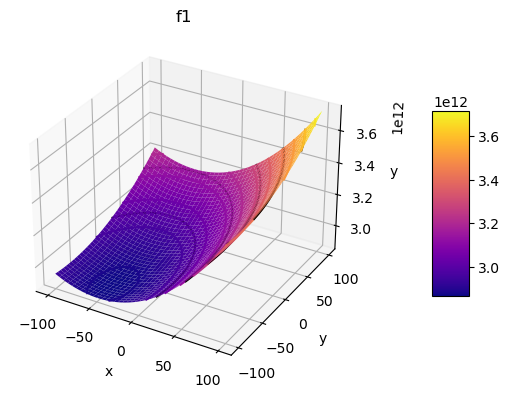
\includegraphics[width=\linewidth]{figuras/funciones_cec2017/shifted_rotated_f1.png}
        \caption{\(f_1\): función unimodal \textit{Bent Cigar}.}
    \end{subfigure}
    \hfill
    \begin{subfigure}[t]{0.45\textwidth}
        \centering
        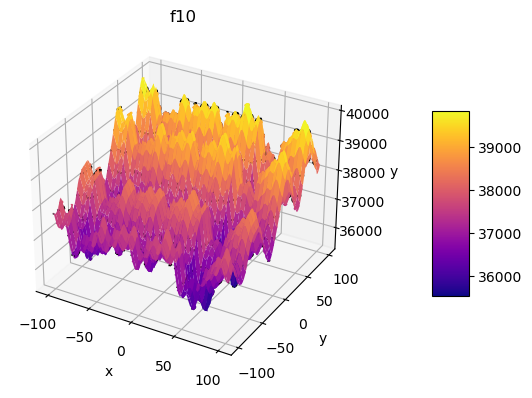
\includegraphics[width=\linewidth]{figuras/funciones_cec2017/f10.png}
        \caption{\(f_{10}\): función multimodal \textit{Schwefel}.}
    \end{subfigure}
    \caption{Representación ilustrativa de dos paisajes de
        búsqueda pertenecientes a la suite CEC2017.}
    \label{fig:paisajes_cec2017}
\end{figure}

La suite fue definida inicialmente con \textbf{30 funciones}, aunque revisiones posteriores eliminaron \(f_2\) debido a su inestabilidad numérica. En este trabajo, consideramos la suite completa ya que es la expuesta por la implementación empleada.

\begin{table}[H]
    \centering
    \begin{tabular}{lc}
        \toprule
        \textbf{Familia}     & \textbf{Funciones}     \\
        \midrule
        Unimodales           & \(f_1\)--\(f_3\)       \\
        Multimodales simples & \(f_4\)--\(f_{10}\)    \\
        Híbridas             & \(f_{11}\)--\(f_{20}\) \\
        Compuestas           & \(f_{21}\)--\(f_{30}\) \\
        \bottomrule
    \end{tabular}
    \caption{Familias de funciones de CEC2017 según la numeración empleada en este trabajo.}
    \label{tab:familias_cec2017}
\end{table}

Los detalles concretos de la integración software del benchmark y de la
interfaz de evaluación empleada se recogen en la
Sección~\ref{sec:detalles_implementacion}.

% \subsection{Funciones consideradas en cada fase experimental}

% % Distingue entre la suite completa y el subconjunto representativo utilizado para el cribado y el ajuste fino.

% El uso de CEC2017 se adapta a los objetivos y al coste computacional de cada
% fase experimental. Para analizar el comportamiento de las metaheurísticas y
% evaluar las distintas configuraciones del mecanismo de reinicio elitista se
% utilizan las \textbf{30 funciones} expuestas por la implementación empleada. Esta evaluación permite comprobar la robustez de cada configuración sobre paisajes de búsqueda diversos antes de generar las trayectorias destinadas al estudio de los modelos subrogados.

% Dado el elevado coste computacional que supondría ejecutar múltiples combinaciones de modelos, estrategias de entrenamiento y semillas sobre el benchmark completo, esta fase se realiza sobre un subconjunto fijo de \textbf{siete funciones} seleccionadas para cubrir las cuatro familias descritas anteriormente:

% 
\begin{table}[H]
    \centering
    \begin{adjustbox}{max width=0.55\textwidth}
        \begin{tabular}{lc}
            \toprule
            \textbf{Familia} & \textbf{Funciones} \\
            \midrule
            Unimodales       & \(f_1\)            \\
            Multimodales     & \(f_4, f_{10}\)    \\
            Híbridas         & \(f_{12}, f_{18}\) \\
            Compuestas       & \(f_{22}, f_{29}\) \\
            \bottomrule
        \end{tabular}
    \end{adjustbox}
    \caption{Funciones seleccionadas para la evaluación inicial de las técnicas subrogadas.}
    \label{tab:funciones_cribado_surrogate}
\end{table}

% Este subconjunto permite identificar los modelos y las estrategias de
% entrenamiento más prometedores antes de abordar las fases posteriores del
% estudio, reservando la validación sobre el benchmark
% completo para las configuraciones finales que superen con éxito esta fase de
% cribado.

%%%%%%%%%%%%%%%%%%%%%%
\section{Estrategias de resolución: Metaheurísticas}
\label{sec:metaheuristicas}

% Expone las condiciones bajo las que AGE, DE y SHADE generan las trayectorias.


% Indica dimensión, dominio, presupuesto de evaluaciones, tamaño de población y semillas.

% Recoge en tablas los parámetros específicos de cada algoritmo.

Las metaheurísticas AGE, DE y SHADE, descritas en el
Capítulo~\ref{chap:algo_tecnicas_ref}, se ejecutan bajo las mismas condiciones
con el objetivo de obtener historiales de evaluaciones comparables. Todas las pruebas
se realizan en dimensión \(D=10\), sobre el dominio de búsqueda
\([-100,100]^{10}\), y utilizan un tamaño de población fijo de \textbf{50 individuos.}

El criterio de parada se establece mediante el número de evaluaciones de la
función objetivo. Siguiendo la definición propia de CEC2017, cada ejecución
dispone de un presupuesto máximo de \(10000 \cdot D\) evaluaciones. Por tanto,
al considerar \(D=10\), el límite se fija en \(100000\) evaluaciones por
ejecución.

Dado que las metaheurísticas consideradas incorporan \textbf{componentes aleatorias}, una única ejecución no resulta suficiente para valorar su comportamiento. Por este motivo, cada combinación de función y metaheurística se ejecuta un total de \textbf{\(51\) veces}.

\begin{table}[H]
    \centering
    \begin{adjustbox}{max width=\textwidth}
        \begin{tabular}{lc}
        \toprule
        \textbf{Parámetro}                   & \textbf{Valor}            \\
        \midrule
        Dimensión del problema               & \(D=10\)                  \\
        Dominio de búsqueda                  & \([-100,100]^{10}\)       \\
        Presupuesto máximo de evaluaciones   & \(100000\)                \\
        Tamaño de la población               & \(50\)                    \\
        Número de ejecuciones independientes & \(51\)                    \\
        \bottomrule
        \end{tabular}
    \end{adjustbox}
    \caption{Parámetros comunes utilizados en la ejecución de las
        metaheurísticas.}
    \label{tab:parametros_comunes_metaheuristicas}
\end{table}


A partir del entorno de evaluación definido, cada metaheurística mantiene la
configuración propia de su esquema de búsqueda. Los operadores y particularidades de los
algoritmos se desarrollaron en el Capítulo~\ref{chap:algo_tecnicas_ref}, por lo
que a continuación se recogen únicamente los valores utilizados durante la
generación del histórico de evaluaciones.

\begin{enumerate}
    \item \textbf{AGE:} para la implementación propia se utilizan los parámetros recogidos en la Tabla~\ref{tab:parametros_age}.

          \begin{table}[htbp]
              \centering
              \begin{adjustbox}{max width=\textwidth}
                  \begin{tabular}{lc|lc}
                      \toprule
                      \textbf{Parámetro}                              & \textbf{Valor} &
                      \textbf{Parámetro}                              & \textbf{Valor}   \\
                      \midrule
                      \textbf{Tamaño del torneo}                      & \(2\)          &
                      \textbf{Probabilidad de cruce}                  & \(0.7\)          \\
                      \textbf{Probabilidad de mutación}               & \(0.1\)        &
                      \textbf{Parámetro \(\alpha\) de BLX-\(\alpha\)} & \(0.45\)         \\
                      \textbf{Desviación típica de la mutación}       & \(0.3\)        &
                                                                      &                  \\
                      \bottomrule
                  \end{tabular}
              \end{adjustbox}
              \caption{Parámetros utilizados para AGE.}
              \label{tab:parametros_age}
          \end{table}

    \item \textbf{DE:} se emplea la variante DE/rand/1/bin por defecto de la implementación empleada (véase en la
          Tabla~\ref{tab:parametros_de}).

          \begin{table}[htbp]
              \centering
              \begin{adjustbox}{max width=\textwidth}
                  \begin{tabular}{lc|lc}
                      \toprule
                      \textbf{Parámetro}                    & \textbf{Valor} &
                      \textbf{Parámetro}                    & \textbf{Valor}   \\
                      \midrule
                      \textbf{Estrategia de mutación}       & DE/rand/1      &
                      \textbf{Operador de cruce}            & Binomial         \\
                      \textbf{Factor de escala \(F\)}       & \(0.5\)        &
                      \textbf{Probabilidad de cruce \(CR\)} & \(0.9\)          \\
                      \bottomrule
                  \end{tabular}
              \end{adjustbox}
              \caption{Parámetros utilizados para DE.}
              \label{tab:parametros_de}
          \end{table}

    \item \textbf{SHADE:} se mantiene la configuración por defecto de la implementación empleada (véase en
          la Tabla~\ref{tab:parametros_shade}).

          \begin{table}[htbp]
              \centering
              \begin{adjustbox}{max width=\textwidth}
                  \begin{tabular}{lc|lc}
                      \toprule
                      \textbf{Parámetro}                    & \textbf{Valor}     &
                      \textbf{Parámetro}                    & \textbf{Valor}       \\
                      \midrule
                      \textbf{Estrategia de mutación}       & current-to-pbest/1 &
                      \textbf{Operador de cruce}            & Binomial             \\
                      \textbf{Factor de escala \(F\)}       & Adaptativo         &
                      \textbf{Probabilidad de cruce \(CR\)} & Adaptativa           \\
                      \textbf{Tam. de la mem. histórica}    & \(100\)            &
                                                            &                      \\
                      \bottomrule
                  \end{tabular}
              \end{adjustbox}
              \caption{Parámetros utilizados para SHADE.}
              \label{tab:parametros_shade}
          \end{table}

\end{enumerate}


\subsection{Criterio de reinicio elitista}
\label{subsec:criterio_reinicio}

Para identificar situaciones de \textbf{estancamiento}, se utilizan gráficas de convergencia y diversidad. Si se detecta este comportamiento, se incorpora el mecanimos de reinicio descrito en el Capítulo~\ref{chap:algo_tecnicas_ref}, parametrizado medienta una ventana de estancamiento $\rho$ que expresa, como \textbf{proporción del presupuesto total de evaluaciones}, el tiempo sin mejoras a partir del cual se considera que el algoritmo ha convergido prematuramente.

Tal y como está definido, es necesario definir el criterio de activación, y por tanto, determinar cuándo una variación del segundo mejor individuo se corresponde con una mejora efectiva. Dado que CEC2017 considera nulos los valores por debajo de $10^{-8}$, cualquier variación de \textit{fitness} de menor orden corresponde a ruido numérico. Para descartarlas sin filtrar progresos reales, se contabilizan como mejora únicamente aquellas variaciones cuya magnitud supere una \textbf{tolerancia} de $10^{-6}$.

El impacto de este mecanismo sobre la búsqueda se evalúa con un conjunto de configuraciones del criterio frente a la versión \textit{base} sin reinicio, correspondiente a valores de $\rho$ del $1\%$, $3\%$, $5\%$, $7\%$ y $10\%$.

El análisis se realiza de forma \textbf{independiente} por cada algoritmo ya que el objetivo no es comparar AGE, DE y SHADE entre sí, sino determinar qué configuración de cada uno resulta más adecuada para generar un históral de evaluaciones útil en la fase subrogada. Para ello, se utiliza el \textbf{ranking medio}, agregando los resultados sobre todas las funciones sin que las de mayor magnitud de error distorsionen la agregación.

%%%%%%%%%%%%%%%%%%%%%%
\section{Registro temporal de evaluaciones}
\label{sec:generacion_trayectorias}

Durante la ejecución de las metaheurísticas se registran cronológicamente las
evaluaciones reales realizadas sobre la función objetivo.

En lugar de analizar únicamente el resultado final de cada ejecución, este trabajo utiliza la secuencia temporal de soluciones evaluadas para estudiar cómo evoluciona la información disponible a lo largo de la búsqueda y cómo puede aprovecharse posteriormente en la fase de evaluación subrogada sobre el histórico de datos.

Para cada evaluación se registra el vector de decisión
\(\mathbf{x} \in \mathbb{R}^{D}\), el valor real de \textit{fitness} obtenido al
evaluar la función objetivo y un \textbf{identificador temporal} que indica el orden en el que se generó la muestra. La Tabla~\ref{tab:estructura_trayectorias}
resume la información registrada y su utilidad posterior.

\begin{table}[H]
    \centering
    \begin{tabular}{l p{9.4cm}}
        \toprule
        \textbf{Campo} & \textbf{Descripción}                                                                                            \\
        \midrule
        \texttt{eval\_id}
                       & Identificador que refleja el orden cronológico de evaluación para la posterior partición en bloques temporales. \\
        \midrule
        \(\mathbf{x}\)
                       & Vector de decisión asociado a la solución candidata.                                                            \\
        \midrule
        \textit{fitness}
                       & Valor real obtenido al evaluar la función objetivo.                                                             \\
        \bottomrule
    \end{tabular}
    \caption{Información registrada para cada evaluación.}
    \label{tab:estructura_trayectorias}
\end{table}

A partir de este histórico de evaluaciones, cada ejecución se organiza posteriormente en bloques temporales que permiten construir los conjuntos de entrenamiento y validación empleados en la evaluación posterior de los modelos subrogados.

%%%%%%%%%%%%%%%%%%%%%%
\section{Técnicas subrogadas: modelos candidatos y de referencia}

Los modelos empleados en este trabajo se presentaron conceptualmente en el Capítulo~\ref{chap:algo_tecnicas_ref}. Esta sección se centra en cómo se preparan los datos antes de entrenar cada modelo y qué configuración concreta se utiliza en la Sección~\ref{subsec:comparacion_modelos}.

\subsection{Configuración experimental de los modelos}

Como se comentó en la Sección \ref{sec:tecnicas_subrogadas}, Kriging y
PCE se incorporan como técnicas clásicas de referencia, por lo que no forman
parte del mismo protocolo experimental aplicado inicialmente al resto de
regresores.

Para garantizar una comparación no sobreajustada a los problemas de optimización de CEC2017, metaheurística o semilla, se mantienen algunos parámetros en sus valores por defecto y se modifican los que sí merecen ser ajustados para evitar comportamientos sesgados. La configuración no predeterminada empleada en cada modelo se recoge en la Tabla~\ref{tab:surrogate_models_config}.

%% hay que cambiar la implementacion de pce

\begin{table}[htbp]
    \centering
    \begin{tabular}{l p{7cm}}
        \toprule
        \textbf{Modelo} & \textbf{Configuración no predeterminada}                                                \\
        \midrule
        LASSO           & \makecell[l]{\texttt{alpha=0.01}                                                        \\ \texttt{max\_iter=5000} \\ \texttt{random\_state=42}} \\
        \midrule
        RSM             & \texttt{PolynomialFeatures} sobre regresión lineal ordinaria. Configuración por defecto \\
        \midrule
        RBF             & \makecell[l]{\texttt{neighbors=50}                                                      \\ \texttt{smoothing=1} \\ \texttt{kernel=gaussian} \\ \texttt{degree=-1} \\ \texttt{epsilon=1.0}} \\
        \midrule
        SVR             & Configuración por defecto                                                               \\
        \midrule
        MLP             & \makecell[l]{\texttt{hidden\_layer\_sizes=(128,\,64)}                                   \\ \texttt{alpha=1e-3} \\ \texttt{max\_iter=2000} \\ \texttt{random\_state=42} \\ \texttt{early\_stopping=True}} \\
        \midrule
        Random Forest   & \makecell[l]{\texttt{n\_estimators=200}                                                 \\ \texttt{max\_depth=16} \\ \texttt{min\_samples\_leaf=5} \\ \texttt{max\_features=0.5} \\ \texttt{random\_state=42} \\ \texttt{n\_jobs=-1}} \\
        \midrule
        HGB             & \makecell[l]{\texttt{max\_iter=200}                                                     \\ \texttt{learning\_rate=0.05} \\ \texttt{max\_depth=4} \\ \texttt{l2\_regularization=1e-3} \\ \texttt{random\_state=42}} \\
        \midrule
        XGBoost         & \makecell[l]{\texttt{n\_estimators=400}                                                 \\ \texttt{max\_depth=4} \\ \texttt{learning\_rate=0.05} \\ \texttt{subsample=0.8} \\ \texttt{colsample\_bytree=0.8} \\ \texttt{random\_state=42} \\ \texttt{n\_jobs=-1} \\ \texttt{tree\_method=hist}} \\
        \midrule
        Kriging         & \texttt{corr=matern52}                                                                  \\
        \midrule
        PCE             & \texttt{order=3}                                                                        \\
        \bottomrule
    \end{tabular}
    \caption{Configuración inicial empleada para la evaluación de los modelos subrogados.}
    \label{tab:surrogate_models_config}
\end{table}

\subsection{Preprocesamiento de los datos}
\label{subsec:preprocesamiento}

Antes de entrenar cada modelo, los datos generados por las distintas metaheurísticas requieren dos \textbf{transformaciones independientes} que afectan, respectivamente, a las variables de entrada y a la variable objetivo.

\textbf{Escalado de las variables de entrada.} Para mantener un protocolo homogéneo y robusto entre modelos, \textbf{todas las técnicas} se entrenan con las variables de entrada escaladas. Esta transformación es especialmente importante en técnicas sensibles a la magnitud de las variables, como LASSO, MLP, SVR, RBF y RSM. Aunque no es estrictamente necesario para el resto, se mantiene también en estos casos para mantener la consistencia del procedimiento experimental. Dado que en \textbf{CEC2017} las variables de decisión se definen sobre el dominio \([-100,100]^{D}\), todas las muestras se reescalan al intervalo \([-1,1]^{D}\) mediante la transformación \[
    x_{j}^{\ast} = \frac{x_{j}}{100}.
\]
De este modo, se evitan diferencias de escala innecesarias entre variables y se aplica el mismo preprocesamiento a todos los modelos considerados.

\textbf{Escalado de la variable objetivo.} En algunos modelos, la escala de la variable objetivo puede influir directamente en el ajuste. Por este motivo, se estandiraza el valor de \textit{fitness} únicamente en aquellos modelos donde resulta necesario: LASSO, RSM, RBF, SVR y MLP. En estos casos, y a partir de las formulaciones matemáticas de cada modelo definidas en el Capítulo~\ref{chap:algo_tecnicas_ref}, la magnitud de \(y\) puede afectar a la regularización, al condicionamiento numérico o al proceso de optimización interno del modelo.

Para los modelos en los que sí se estandariza la variable objetivo, se utiliza la transformación
\[
    y^{\ast} = \frac{y - \mu_{y}}{\sigma_{y}}, \qquad
    \mu_{y} = \frac{1}{n}\sum_{i=1}^{n} y_{i}, \qquad
    \sigma_{y} = \sqrt{\frac{1}{n}\sum_{i=1}^{n} (y_{i} - \mu_{y})^{2}}.
\]
Los valores $\mu_{y}$ y $\sigma_{y}$ se calculan \textbf{exclusivamente sobre el conjunto de entrenamiento}, evitando así filtraciones de información (\textit{data leakage}) desde el conjunto de validación. Tras la predicción, el resultado se devuelve a la escala original del problema mediante la \textbf{transformación inversa}, de forma que todos los modelos se comparan sobre los valores reales de  \textit{fitness}.

\section{Métricas empleadas}

Para evaluar el rendimiento de los modelos subrogados se utilizan distintas métricas que podemos agrupar en tres familias complementarias: el \textbf{error de predicción}, la \textbf{capacidad de ordenación} y el \textbf{coste computacional}.

\subsection{Error de predicción}

La capacidad de predicción de un modelo determina su calidad como regresor.
Para cuantificarla se emplean el \textbf{error absoluto medio} (MAE) y la
\textbf{raíz del error cuadrático medio} (RMSE), junto con sus correspondientes
versiones normalizadas.

Dado un conjunto de validación formado por \(n\) pares
\(\{(\mathbf{x}_i, y_i)\}_{i=1}^{n}\), donde \(y_i\) es el valor real del
\textit{fitness} y \(\hat{f}(\mathbf{x}_i)\) la predicción del modelo, ambas
métricas se definen como


\begin{equation}
    \text{MAE} = \frac{1}{n}\sum_{i=1}^{n} \bigl|y_i - \hat{f}(\mathbf{x}_i)\bigr|,
    \label{eq:mae}
\end{equation}

\begin{equation}
    \text{RMSE} = \sqrt{\frac{1}{n}\sum_{i=1}^{n} \bigl(y_i - \hat{f}(\mathbf{x}_i)\bigr)^2}.
    \label{eq:rmse}
\end{equation}

La diferencia entre ambas es la \textbf{sensibilidad al penalizar errores de mayor magnitud}. A diferencia del MAE, el RMSE penaliza con mayor intensidad \textbf{casos atípicos}, por lo que resulta muy útil para detectar fallos puntuales relevantes.

Dado que las funciones de CEC2017 presentan rangos de \textit{fitness} muy distintos, los valores absolutos de MAE y RMSE no resultan comparables entre funciones ni entre bloques temporales de una mismo histórico de evaluaciones. Para facilitar su interpretación, ambas se normalizan dividiéndolas por la media de los valores absolutos del \textit{fitness} real en el conjunto de validación, denotada como \(\bar{|y|} = \frac{1}{n}\sum_{i=1}^{n}|y_i|\):

\begin{equation}
    \text{NMAE} = \frac{\text{MAE}}{\bar{|y|}},
    \label{eq:nmae}
\end{equation}

\begin{equation}
    \text{NRMSE} = \frac{\text{RMSE}}{\bar{|y|}}.
    \label{eq:nrmse}
\end{equation}

En este caso, los valores próximos a cero indican que las predicciones se
mantienen cercanas a los valores reales de \textit{fitness}.

\subsection{Capacidad de ordenación}

Como se expuso en la
Sección~\ref{subsec:clasificacion_surrogates_prediccion}, la utilidad de un
modelo subrogado dentro de una metaheurística no depende únicamente de su
precisión numérica. Un modelo subrogado puede realizar predicciones que no son precisas pero puede ser capaz de ordenar correctamente las soluciones candidatas.

Para evaluar esta propiedad se
emplea el \textbf{coeficiente de correlación de Spearman}, que cuantifica el grado de concordancia ordinal
entre los valores reales y los predichos.

El coeficiente se calcula como la correlación de Pearson aplicada a los rangos de ambas distribuciones. Sea \(R_i\) el rango del valor real del \textit{fitness} de la muestra \(i\) dentro del conjunto de validación, y \(Q_i\) el rango de la predicción correspondiente. Entonces:

\begin{equation}
    \rho_s
    =
    \frac{
        \displaystyle\sum_{i=1}^{n}
        (R_i - \bar{R})(Q_i - \bar{Q})
    }{
        \sqrt{
            \displaystyle\sum_{i=1}^{n}(R_i - \bar{R})^2
            \cdot
            \displaystyle\sum_{i=1}^{n}(Q_i - \bar{Q})^2
        }
    },
    \label{eq:spearman}
\end{equation}
donde \(\bar{R}\) y \(\bar{Q}\) son los rangos medios.

El coeficiente toma valores en \([-1, 1]\). Un valor \(1\) indica concordancia perfecta de orden, \(-1\) refleja un orden completamente invertido, y \(0\) señala ausencia de relación ordinal.

Cuando dos o más valores coinciden, se les asignan rangos consecutivos según
su orden de aparición en el vector correspondiente. De este modo, incluso si
un subrogado genera predicciones constantes, se mantiene una ordenación total
determinista y el coeficiente puede calcularse de forma consistente entre
ejecuciones.

% En la implementación, los rangos se obtienen mediante
% \texttt{scipy.stats.rankdata(\ldots, method="ordinal")} y posteriormente se
% calcula la correlación entre dichos rangos mediante \texttt{scipy.stats.pearsonr}.

\subsection{Coste computacional}

La viabilidad de un modelo subrogado para la hibridación también depende de su coste computacional:

\begin{itemize}
    \item \textbf{Tiempo de entrenamiento:} tiempo necesario, en segundos, para ajustar el modelo sobre el conjunto de entrenamiento.
    \item \textbf{Tiempo de predicción:} tiempo requerido, en segundos, para evaluar el modelo sobre las muestras del conjunto de validación.
\end{itemize}

Un modelo con un tiempo de entrenamiento elevado puede no ser adecuado si debe reajustarse varias veces durante la ejecución. Del mismo modo, un tiempo de predicción alto reduce la ventaja de usar el subrogado para filtrar candidatos antes de realizar evaluaciones reales. Por tanto, ambos deben analizarse conjuntamente para identificar configuraciones cuyo coste pueda comprometer su posterior integración.

\subsection{Criterio de comparación de los modelos}
\label{subsec:criterio_comparacion_modelos}

A lo largo de este trabajo, la comparación entre modelos se realiza analizando conjuntamente las métricas anteriores. Estas se presentan a continuación en orden de importancia:

\begin{enumerate}
    \item \textbf{Coeficiente de Spearman:} permite valorar si el subrogado preserva el orden relativo de calidad entre las soluciones candidatas.
    \item \textbf{Coste computacional:} analiza la viabilidad para la posterior hibridación.
          \begin{enumerate}
              \item \textbf{Tiempo de predicción}
              \item \textbf{Tiempo de entrenamiento}
          \end{enumerate}
    \item \textbf{NMAE y NRMSE:} se emplean como métricas complementarias para evaluar la calidad predictiva ya que no es el objetivo de este trabajo.
\end{enumerate}

%%%%%%%%%%%%%%%%%%%%%%
\section{Evaluación de modelos subrogados sobre históricos de evaluaciones}

Los datos de búsqueda generados por las metaheurísticas se organizan en \textbf{cinco bloques temporales consecutivos}, cada uno de ellos correspondiente al \textbf{20\,\% del presupuesto total de evaluaciones}. Dado que cada ejecución comprende \(100\,000\) evaluaciones, cada bloque agrupa \(20\,000\) muestras, ordenadas cronológicamente según el instante en que fueron generadas durante la búsqueda. Los bloques se identifican por el intervalo porcentual que ocupan dentro de las evaluaciones realizadas: \textbf{1--20\,\%}, \textbf{21--40\,\%}, \textbf{41--60\,\%}, \textbf{61--80\,\%} y \textbf{81--100\,\%}.

A partir de esta partición, las dos estrategias definidas en la
Sección~\ref{sec:metodologia_estrategias_offline} se instancian en este trabajo mediante los
conjuntos de entrenamiento recogidos en la
Tabla~\ref{tab:pares_entrenamiento_validacion}. La \textbf{estrategia no acumulativa} utiliza un único bloque en cada ajuste, mientras que la \textbf{acumulativa} incorpora progresivamente todos los bloques disponibles hasta el instante considerado.

\begin{table}[H]
    \centering
    \renewcommand{\arraystretch}{1.15}
    \begin{adjustbox}{max width=\textwidth}
        \begin{tabular}{c|c c|c c|c}
            \toprule
            \multirow{2}{*}{\textbf{Bloque}} & \multicolumn{2}{c|}{\textbf{No acumulativa}} & \multicolumn{2}{c|}{\textbf{Acumulativa}}                                                & \multirow{2}{*}{\makecell{\textbf{Bloque}                                  \\\textbf{de validación}}} \\
            \cmidrule(lr){2-3} \cmidrule(lr){4-5}
                                             & Intervalo                                    & \makecell{\textbf{Tamaño}                                                                                                                                             \\ \textbf{entrenamiento}} & Intervalo & \makecell{\textbf{Tamaño} \\ \textbf{entrenamiento}} & \\
            \midrule
            $B_1$                            & 1--20\,\%                                    & 20\,000                                                                                  & 1--20\,\%                                 & 20\,000 & $B_2$\ (21--40\,\%)  \\
            $B_2$                            & 21--40\,\%                                   & 20\,000                                                                                  & 1--40\,\%                                 & 40\,000 & $B_3$\ (41--60\,\%)  \\
            $B_3$                            & 41--60\,\%                                   & 20\,000                                                                                  & 1--60\,\%                                 & 60\,000 & $B_4$\ (61--80\,\%)  \\
            $B_4$                            & 61--80\,\%                                   & 20\,000                                                                                  & 1--80\,\%                                 & 80\,000 & $B_5$\ (81--100\,\%) \\
            $B_5$                            & 81--100\,\%                                  & \multicolumn{4}{c}{\cellcolor{gray!10}\textbf{Reservado exclusivamente para validación}}                                                                              \\
            \bottomrule
        \end{tabular}
    \end{adjustbox}
    \caption{Resumen de las particiones utilizadas para construir los conjuntos de entrenamiento y validación en ambas estrategias.}
    \label{tab:pares_entrenamiento_validacion}
\end{table}

Como se observa en la tabla, el bloque~5 queda reservado exclusivamente para validación al no haber más muestras sobre las que validar el modelo si utilizase dicho bloque como entrenamiento.

Para que los resultados sean comparables y no dependan del tamaño del conjunto de entrenamiento empleado, el conjunto de validación se toma siempre del bloque temporal inmediatamente posterior al último bloque utilizado para entrenar el mdoelo. Como cada bloque contiene \(20000\)
evaluaciones, se selecciona el \textbf{25\% de sus muestras}, es decir, \textbf{5000 soluciones} evaluadas por ejecución. Este criterio se aplica tanto en la estrategia acumulativa como en la no acumulativa, de forma que el tamaño del conjunto de validación no depende del número de bloques empleadas en el entrenamiento.

La selección de las muestras se realiza de forma determinista a partir de la semilla de la ejecución y del bloque temporal utilizado para validación. De esta forma, para una misma ejecución y un mismo bloque, el conjunto de validación queda fijado y es común a todos los modelos y estrategias evaluados.

Dado el coste computacional de evaluar todas las combinaciones de modelos, estrategias de entrenamiento y semillas sobre la suite completa, la primera comparación se realiza sobre un subconjunto de funciones de CEC2017. En esta fase se mantienen las \(51\) semillas empleadas en las ejecuciones de las metaheurísticas, pero se reduce el número de funciones para hacer viable la comparación inicial entre modelos.

El subconjunto se elige para cubrir las principales familias de funciones del benchmark:

\begin{itemize}
    \item \textbf{Unimodal:} \(f_1\).
    \item \textbf{Multimodal:} \(f_4\), \(f_{10}\).
    \item \textbf{Híbrida:} \(f_{12}\), \(f_{18}\).
    \item \textbf{Compuesta:} \(f_{22}\), \(f_{29}\).
\end{itemize}

Con esta selección se comparan los modelos en funciones con características distintas, sin elevar innecesariamente el coste experimental. Las configuraciones seleccionadas en esta fase se evalúan posteriormente sobre la suite completa.

%%%%%%%%%%%%%%%%%%%%%%
\section{Ajuste fino de hiperparámetros}
\label{sec:protocolo_ajuste_hiperparametros}

%% objetivo del ajuste fino: Explicar que no se busca rediseñar todos los modelos, sino refinar los hiperparámetros de los modelos candidatos tras el cribado offline

% idea clave: El ajuste fino no constituye una nueva fase de comparación global entre todos los regresores, sino una optimización acotada de los modelos que hayan mostrado mejor comportamiento en la fase offline.

El ajuste fino de hiperparámetros se plantea como una fase posterior a la decisión de la mejor estrategia y la comparación inicial de modelos. Su objetivo no es repetir la comparación completa entre todos los regresores, sino refinar la configuración de aquellos que hayan obtenido mejores resultados antes de evaluarlos sobre la suite completa. De esta forma, el coste experimental se concentra en el modelo o modelos con mayor probabilidad de resultar útiles en una posterior integración.

Dado que el coste de entrenamiento y predicción no es el mismo para todos los modelos, el número de semillas usado en esta fase puede variar según la técnica considerada. Cuando dicho coste sea elevado, el ajuste se realizará sobre un subconjunto fijo de semillas para que la búsqueda de hiperparámetros sea asumible.
Esta reducción afecta únicamente a la fase de ajuste, ya que la configuración o configuraciones finalmente seleccionadas se comparan posteriormente sobre las \(30\) funciones de CEC2017
y las \(51\) semillas empleadas para el histórico de evaluaciones.

El procedimiento mantiene el orden temporal de los datos generados por cada metaheurística. Para evitar que la elección de hiperparámetros utilice información posterior al bloque de entrenamiento (\textit{data leakage}), se aplica una partición interna dentro de dicho bloque:

\begin{itemize}
    \item El \textbf{80\% inicial} de las muestras del bloque se utiliza para el entrenamiento de las distintas configuraciones candidatas que componen el espacio de búsqueda.
    \item El \textbf{20\% final} de dicho bloque se reserva como conjunto de validación interna para evaluar el rendimiento de cada configuración y estimar su capacidad de generalización dentro de la misma etapa temporal.
\end{itemize}

Una vez elegida la configuración, el modelo se reentrena con todas las muestras del bloque de entrenamiento y se evalúa sobre un subconjunto del bloque temporal inmediatamente posterior (conjunto de validación). Así, las muestras futuras no intervienen en la selección de hiperparámetros, sino solo en la evaluación del modelo ya ajustado.

La Figura~\ref{fig:ajuste_hiperparametros_validacion_interna} representa este
procedimiento para una transición concreta. En el ejemplo, el ajuste interno
se realiza sobre el bloque correspondiente al intervalo 20--40\% de la
búsqueda y la evaluación posterior utiliza muestras pertenecientes al
intervalo 40--60\%.


\begin{figure}[H]
    \centering
    \begin{tikzpicture}[
            scale=0.9,
            every node/.style={transform shape},
            bloque/.style={draw, minimum height=0.9cm, font=\footnotesize, align=center, inner sep=3pt},
            flecha/.style={->, thick}
        ]

        % Nodo de entrenamiento (superior)
        \node[bloque, minimum width=2.2cm, fill=blue!10] (train) at (0,0)
        {80\%\\Ajuste};
        % Nodo de validación interna, justo debajo
        \node[bloque, minimum width=1.3cm, fill=orange!15, below=1.0cm of train] (valint)
        {20\%\\Val.};

        % Etiqueta de etapa temporal arriba, centrada respecto ambos nodos
        \node[font=\footnotesize, above=0.42cm of train]
        {\textbf{Entrenamiento 20--40\%}};

        % Selección de hiperparámetros a la derecha, alineada verticalmente con train
        \node[bloque, minimum width=1.7cm, fill=gray!10, right=2.0cm of train] (select)
        {Selec.\\Hiperparam.};
        % Futuro a la derecha del anterior
        \node[bloque, minimum width=1.7cm, fill=green!12, right=1.7cm of select] (future)
        {Futuro\\40--60\%};

        % Flechas de proceso
        \draw[flecha] (train.east) -- (select.west);
        \draw[flecha] (valint.east) -- ([yshift=0.0cm]select.south west);

        % Unión de validación interna hacia la selección de hiperparámetros (desde la derecha de valint hacia abajo del bloque de selección)
        % Flecha de proceso hacia el futuro
        \draw[flecha] (select.east) -- (future.west);

    \end{tikzpicture}
    \caption[Esquema de validación interna para el ajuste de hiperparámetros]{Esquema de validación interna para el ajuste de hiperparámetros con los conjuntos de ajuste y validación dispuestos en paralelo.}
    \label{fig:ajuste_hiperparametros_validacion_interna}
\end{figure}

% Ajustes recomendados: scale ~0.80, fuente \footnotesize, minimum width y height menores, distancias proporcionadas.

La búsqueda de hiperparámetros se realiza de forma exhaustiva sobre un espacio acotado de valores definido y la selección final sigue el criterio definido en la Subsección~\ref{subsec:criterio_comparacion_modelos}.

Las configuraciones consideradas para los modelos finalistas se presentan junto con
sus resultados en el capítulo siguiente.

\section{Integración del modelo subrogado durante la búsqueda}
\label{sec:integracion_subrogado_busqueda}

La integración del modelo subrogado durante la búsqueda se evalúa mediante el mecanismo de filtrado definido en la Sección~\ref{sec:estrategia_online_integracion_surrogate}. En esta fase, a diferencia de la evaluación sobre históricos de evaluaciones, las predicciones del subrogado pueden modificar las decisiones de la metaheurística. Por tanto, la comparación ya no se limita a medir la calidad de ordenación del modelo, sino que trata la hibridación como una variante del algoritmo original.

Para mantener acotado el coste experimental, la integración no se aplica a todos los modelos candidatos. Solo se considera el modelo y la estrategia de entrenamiento seleccionados tras la evaluación previa y el ajuste de hiperparámetros. El objetivo es comprobar si el subrogado elegido mejora el comportamiento de la metaheurística cuando interviene directamente en el proceso de búsqueda, tomando como referencia la versión original sin subrogado.

A partir de este esquema, el protocolo de integración queda definido por las siguientes decisiones experimentales:

\begin{enumerate}
    \item \textbf{Periodo inicial de calentamiento.} El filtro subrogado no se activa desde el inicio, ya que primero es necesario disponer de evaluaciones reales para entrenar el primer modelo y que pueda generar predicciones útiles. Si \(E_{\max}\) es el presupuesto total y \(\alpha_{\text{warm}}\) la proporción reservada a esta fase, el número de evaluaciones iniciales es
          \[
              E_{\text{warm}} = \alpha_{\text{warm}} E_{\max}.
          \]
          En coherencia con la división temporal utilizada en la evaluación previa, este periodo inicial se fija en el \(20\%\) del presupuesto total de evaluaciones (\(\alpha_{\text{warm}}=0.20\)).

    \item \textbf{Conjunto de entrenamiento.} El modelo se entrena únicamente con evaluaciones reales ya
          observadas. La construcción de este conjunto mantiene el orden temporal
          de la búsqueda y queda determinada por la estrategia de entrenamiento
          seleccionada previamente.

    \item \textbf{Frecuencia de actualización.} Para evitar reentrenamientos
          excesivamente frecuentes que supongan un coste computacional excesivo o modelos desfasados, se estudian distintas
          frecuencias de actualización expresadas como proporción del conjunto
          temporal de entrenamiento. Los valores considerados son \(0.25\),
          \(0.50\) y \(0.75\).

    \item \textbf{Probabilidad de uso del filtro.} El subrogado no se consulta necesariamente para todos los candidatos generados. Para cada candidato se extrae \(u \sim \mathcal{U}(0,1)\), y el filtro se aplica solo si
          \[
              u < p_{\text{sub}},
          \]
          donde \(p_{\text{sub}}\) controla la proporción esperada de candidatos sometidos a preevaluación subrogada. Cuando esta condición no se cumple, el candidato sigue el flujo de evaluación real de la metaheurística original.

          Se consideran los valores \(p_{\text{sub}} \in \{0.25, 0.50,
          0.75\}\).

    \item \textbf{Tratamiento tras reinicio.} Después de un reinicio, la
          distribución de soluciones puede cambiar de forma brusca, reduciendo
          temporalmente la representatividad del modelo. Por ello, se evalúa un periodo de enfriamiento durante el cual el filtro permanece desactivado y solo se incorporan evaluaciones reales. Se
          consideran \(50\), \(100\) y \(500\) evaluaciones reales,
          equivalentes a \(1\), \(2\) y \(10\) poblaciones generadas para
          \(N=50\). No se escoge un mayor número de evaluaciones ya que podría ocurrir que el modelo se apagase durante gran parte del proceso de optimización.
\end{enumerate}

Al tratarse como variantes de las metaheurísticas originales, las ejecuciones híbridas mantienen las condiciones generales definidas en la Tabla~\ref{tab:parametros_comunes_metaheuristicas}.

No obstante, para la calibración de los parámetros de integración se emplea un subconjunto reducido de funciones y semillas, distinto al utilizado en las fases previas. Esta fase no busca una optimización exhaustiva, sino tratar de seleccionar una
configuración homogénea para las distintas
metaheurísticas. Por ello, las decisiones experimentales se evalúan sobre las funciones \(f_3\), \(f_5\), \(f_9\), \(f_{15}\), \(f_{19}\), \(f_{24}\) y \(f_{27}\), junto con \(10\) semillas independientes no utilizadas en la selección del modelo.

La comparación entre variantes sigue el criterio agregado definido en la
Sección~\ref{sec:metaheuristicas}, basado en rankings medios sobre CEC2017. Además, se consideran contadores propios de la integración, como el número de reentrenamientos, el tiempo dedicado al modelo y el porcentaje de candidatos rechazados por el filtro.

Una vez seleccionada la configuración, la evaluación final se realiza sobre las \(30\) funciones de CEC2017 y \(51\) semillas nuevas, distintas tanto de las usadas en la calibración como de las empleadas en la evaluación previa. En esta fase, la variante híbrida se compara con la metaheurística original sin intervención subrogada. También se incluyen como referencia las hibridaciones basadas en Kriging y PCE, descritas en la Sección~\ref{sec:tecnicas_subrogadas_clasicas}.

Los resultados de las distintas decisiones experimentales y las comparaciones descritas se presentan en el Capítulo~\ref{chap:experimentacion}.

% Si el subrogado se usa inmediatamente, puede estar entrenado sobre una distribución que ya no representa la nueva población.

% Por ello se introduce un periodo de enfriamiento o cooldown, durante el cual se priorizan evaluaciones reales antes de volver a confiar en el modelo.


% - indicar que la estrategia se evaluara con el modelo seleccionado en el capitulo 7 tras la fase offline y su correspondiente ajuste de hiperparametros


% La selección de la configuración online no se realiza únicamente a partir del menor error medio, sino atendiendo al compromiso entre rendimiento final, robustez entre metaheurísticas y funciones, y coste computacional añadido por el uso del subrogado. Dado que el objetivo es definir una estrategia homogénea de hibridación, se priorizan aquellas configuraciones que presentan buen comportamiento agregado y rankings estables, evitando decisiones condicionadas por una única función o metaheurística.


% Se selecciona una configuración homogénea priorizando el compromiso entre rendimiento final, robustez entre metaheurísticas y coste añadido. Aunque algunas configuraciones obtienen mejores resultados en casos concretos, la combinación cooldown=100, retrain_ratio=0.50 y p=0.50 ofrece el comportamiento agregado más equilibrado para AGE, DE y SHADE. Esta elección evita ajustar la hibridación de forma específica para cada algoritmo y permite evaluar la utilidad general del mecanismo online propuesto.


% La probabilidad de uso del filtro subrogado se ajusta mediante un piloto previo sobre un subconjunto representativo de funciones y semillas, manteniendo fijos el resto de parámetros de la integración. Este piloto no pretende realizar una optimización exhaustiva del hiperparámetro, sino seleccionar un valor robusto y homogéneo para las tres metaheurísticas antes de ejecutar la evaluación completa. Bajo este criterio, se prioriza el comportamiento agregado y el ranking medio frente a mejoras aisladas en una función o algoritmo concreto.

% Los parámetros de la integración online se fijan mediante pilotos previos sobre un subconjunto de funciones y semillas. Esta fase no busca una optimización exhaustiva de hiperparámetros, sino seleccionar una configuración homogénea y computacionalmente viable para las tres metaheurísticas. La evaluación definitiva de dicha configuración se realiza posteriormente sobre la suite completa, utilizando semillas distintas a las empleadas en los pilotos.

% Las semillas empleadas en los pilotos de calibración online se mantienen separadas tanto de las utilizadas en la generación de trayectorias y evaluación offline como de las utilizadas en la evaluación final de la configuración online seleccionada.

% No se incluyó el caso retrain_ratio=1.00, ya que el valor 0.75 ya representa una actualización poco frecuente del modelo y permitió evaluar el efecto de espaciar considerablemente los reentrenamientos. Dado que esta configuración mostró una degradación respecto a 0.50, se descartó ampliar el piloto hacia frecuencias aún menores de actualización, que previsiblemente incrementarían el riesgo de utilizar un modelo desfasado respecto a la región explorada.


% Para la calibración de la estrategia online se consideran tres parámetros específicos: el periodo de enfriamiento tras reinicio, la frecuencia de actualización del modelo y la probabilidad de uso del filtro. Los valores candidatos se recogen en la Tabla~X. Esta fase no pretende realizar una optimización exhaustiva de hiperparámetros, sino seleccionar una configuración homogénea y computacionalmente viable para AGE, DE y SHADE.

%%%%%%%%%%%%%%%%%%%%%%
\section{Detalles de la implementación}
\label{sec:detalles_implementacion}


A diferencia de las secciones anteriores, centradas en definir el protocolo experimental, esta sección recoge las principales decisiones técnicas tomadas para implementar y reproducir los experimentos.


\subsection{Bibliotecas y herramientas empleadas}

La implementación de este trabajo se ha desarrollado en \texttt{Python}, al tratarse de un lenguaje de programación ampliamente utilizado en computación científica, optimización numérica y aprendizaje automático. Gracias a la gran variedad de bibliotecas consolidadas en este ámbito, se homogeniza la integración de las metaheurísticas, modelos subrogados y herramientas de análisis, reduciendo la necesidad de implementar estas componentes desde cero y minimizando posibles errores en el desarrollo.


La integración del benchmark se realiza a partir del repositorio mantenido por Daniel Molina%
\footnote{\url{https://github.com/dmolina/cec2017real}}, basado en el código de referencia de la competición CEC2017 y escrito en \textit{C++}. Sobre este código se ha construido un adaptador común en \textit{Python}, de modo que AGE, DE y SHADE evalúen candidatos mediante una misma interfaz.

Las implementaciones de las metaheurísticas no proceden de una única biblioteca. AGE se ha desarrollado directamente en \textit{Python} a partir del pseudocódigo descrito en el Capítulo~\ref{chap:algo_tecnicas_ref}. En cambio, DE y SHADE parten de las implementaciones de \texttt{PyADE}%
\footnote{\url{https://github.com/xKuZz/pyade}}, que se han adaptado para utilizar la misma infraestructura común que AGE: interfaz de evaluación, registro de históricos e integración del mecanismo de reinicio. De esta forma se aprovechan implementaciones existentes de algoritmos, reduciendo el esfuerzo de desarrollo y manteniendo al mismo tiempo un protocolo homogéneo para las tres metaheurísticas consideradas.

En el caso de los modelos subrogados, la mayoría de los regresores se implementan mediante \textit{scikit-learn}, biblioteca de aprendizaje automático que proporciona una interfaz común para entrenamiento, predicción y ajuste de hiperparámetros. Además, el escalado de la variable objetivo descrito en la Sección~\ref{subsec:preprocesamiento} se realiza mediante \texttt{StandardScaler}, propio de esa misma librería. El modelo RBF se construye con \texttt{RBFInterpolator} de \textit{SciPy}, al ajustarse directamente a la formulación empleada en este trabajo. XGBoost utiliza su biblioteca oficial, ya que las consideradas no cuentan con implementación propia. Por último, Kriging y PCE se implementan mediante \textit{Surrogate Modeling Toolbox} (SMT), una biblioteca especializada en modelado subrogado que permite incorporar estas técnicas clásicas de referencia.

Para describir el comportamiento de estos modelos, las métricas de evaluación se calculan combinando funciones de \textit{scikit-learn}, \textit{SciPy} y \textit{NumPy}. En particular, \textit{scikit-learn} se utiliza para las métricas de error, mientras que \textit{SciPy} y \textit{NumPy} se emplean para las operaciones necesarias en las métricas normalizadas y en el cálculo de la correlación de Spearman.

El procesamiento posterior de los resultados obtenidos por los distintos experimentos combina varias herramientas:

\begin{itemize}
    \item Los ficheros \textbf{HDF5} se gestionan mediante \texttt{PyTables}.
    \item \texttt{pandas} se utiliza
          para agrupar ejecuciones, calcular medias y preparar las tablas del Capítulo~\ref{chap:experimentacion}.
    \item \texttt{Matplotlib} se emplea para generar el soporte visual de los resultados como las curvas de convergencia o de diversidad.
    \item \texttt{DEAP} se usa para el registro de estadísticas
          generacionales, mediante sus utilidades \texttt{Statistics} y \texttt{Logbook}.
    \item La comparación agregada de medias y rankings medios sobre el benchmark se obtiene mediante \textbf{TACOLAB}\footnote{\url{https://tacolab.org/}}, una herramienta web
          orientada al análisis comparativo de algoritmos de optimización.
\end{itemize}

Las versiones concretas de las principales liberías empleadas en el entorno experimental para poder reproducir los experimentos son:

\begin{itemize}
    \item \texttt{Python} 3.14.5
    \item \texttt{NumPy} 2.4.3
    \item \texttt{Matplotlib} 3.10.8
    \item \texttt{SciPy} 1.17.1
    \item \texttt{scikit-learn} 1.8.0
    \item \texttt{SMT} 2.14.0
    \item \texttt{XGBoost} 3.2.0
    \item \texttt{pandas} 3.0.1
    \item \texttt{PyADE} 0.0.2
    \item \texttt{DEAP} 1.4.3
    \item \texttt{PyTables} 3.11.1
\end{itemize}

Adicionalmente, la integración del benchmark CEC2017 requiere compilar el código de referencia escrito en C++. Para ello se han utilizado \texttt{CMake}~4.0.1 y \texttt{Apple Clang}~17.0.0.

\subsection{Registro y almacenamiento de resultados}

Los resultados generados por las metaheurísticas se almacenan de forma independiente para cada combinación de función, algoritmo y semilla en formato \textbf{HDF5 comprimido}, ya que permite manejar eficientemente grandes volúmenes de datos, con un tamaño reducido por la compresión sin perdida y manteniendo separados los distintos experimentos. Además, al conservar los datos en formato numérico, se preserva la precisión asociada al tipo de dato utilizado. El contenido de este fichero se corresponde con el especificado en la Tabla~\ref{tab:estructura_trayectorias}.

Además del fichero principal, durante la ejecución se generan ficheros
\textbf{JSON} y \textbf{CSV} auxiliares con estadísticas descriptivas de la
población, medidas de diversidad y metadatos asociados al mecanismo de
reinicio. Estos archivos no se emplean como variables de entrada para los modelos subrogados, pero sí son útiles para analizar la dinámica de búsqueda y construir gráficas informativas.

El resto de experimentos también genera archivos auxiliares que recogen, para cada función, metaheurística, semilla, bloque y
modelo, las métricas principales, los hiperparámetros empleados y
los tiempos de entrenamiento y predicción. En la integración del modelo subrogado durante la búsqueda, se registra además información específica sobre su uso, como el número de reentrenamientos, el tiempo dedicado al modelo o la proporción de candidatos filtrados.

De este modo, los datos principales de cada ejecución se almacenan en formatos compactos y eficientes y se reservan formatos más ligeros y fáciles de interpretar para el análisis de resultados.

\subsection{Reproducibilidad de los experimentos}

El equipo utilizado para las ejecuciones se corresponde con un MacBook Air, equipado con el procesador Apple M4, que dispone de 10 núcleos distribuidos en 4 de rendimiento y 6 de eficiencia, junto con 16~GB de memoria RAM unificada y el sistema operativo macOS 26.3. Los experimentos se han lanzado de forma \textbf{secuencial}, sin paralelización entre ejecuciones, aunque algunos modelos como Random Forest y XGBoost hacen uso de paralelización interna mediante \texttt{n\_jobs=-1}. Los tiempos de entrenamiento y predicción presentados son directamente comparables dentro del entorno descrito, al haberse obtenido bajo las mismas condiciones de ejecución.

Los experimentos descritos en este capítulo se organizan mediante distintos
programas de ejecución. Cada uno de ellos corresponde a una fase concreta del
estudio y permite modificar los parámetros necesarios sin alterar la
implementación de los algoritmos.

\begin{enumerate}
    \item \textbf{\texttt{ejecutar\_metaheuristicas.py}}: implementa el diseño propuesto en las
          Secciones~\ref{sec:benchmark} y~\ref{sec:metaheuristicas}. Ejecuta las metaheurísticas
          sobre CEC2017 y registra los históricos de evaluaciones descritos en la
          Sección~\ref{sec:generacion_trayectorias}.
    \item \textbf{\texttt{ejecutar\_no\_acumulativo.py}} y \textbf{\texttt{ejecutar\_acumulativo.py}}:
          realizan la evaluación temporal de los modelos subrogados. Ambos comparten los mismos
          parámetros; la diferencia se encuentra en la forma de construir el conjunto de
          entrenamiento, tal y como se describió anteriormente.
    \item \textbf{\texttt{ajustar\_hiperparametros.py}}: lleva a cabo el ajuste fino de
          hiperparámetros conservando la estructura temporal
          e introduciendo una partición interna dentro de cada bloque de entrenamiento.
    \item \textbf{\texttt{ejecutar\_metaheuristicas\_online.py}}: ejecuta las metaheurísticas consideradas sobre CEC2017, incorporando el filtro subrogado y registrando tanto el rendimiento final como los contadores asociados a la hibridación.
\end{enumerate}

Los parámetros de cada programa se recogen en el Apéndice~\ref{ap:parametros_experimentos}.
